\documentclass[a4paper, 12pt]{article}

%\usepackage{cmap}
\usepackage[T2A]{fontenc}
\usepackage[utf8]{inputenc}
\usepackage[english, russian]{babel}
\usepackage{graphicx}
\usepackage[top=1in, bottom=1in, left=3.2cm, right=2.6cm]{geometry}
\graphicspath{./}
\usepackage{biblatex}
\addbibresource{lib.bib}
\linespread{1.5}
\usepackage{ragged2e}
\justifying
\usepackage{listings}
\usepackage{color}
\usepackage{amsmath}


\begin{document}
	
\begin{titlepage}
	\fontsize{12pt}{12pt}\selectfont
	\begin{figure}[t!]
		\centering
		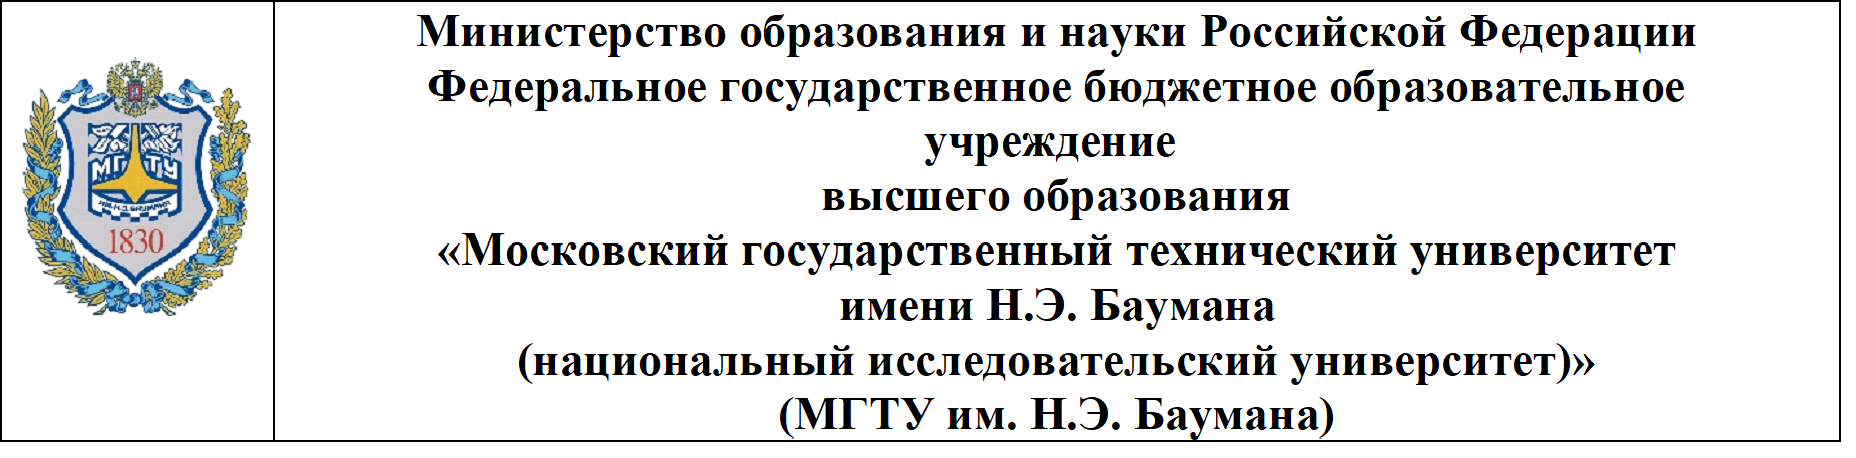
\includegraphics[scale=0.8]{bmstu}
	\end{figure}
	
	\noindent\rule{15cm}{3pt}
	\newline\newline
	\noindent 
	ФАКУЛЬТЕТ 
	\underline{«Информатика и системы управления»} \newline
	
	\noindent КАФЕДРА \underline{«Программное обеспечение ЭВМ и информационные технологии»}\newline\newline\newline\newline\newline
	
	\centering {\Large \textbf{Отчет по лабораторной работе № 4}}
	\vspace{4mm}
	
	\centering {\Large \textbf{По курсу:} Моделирование
		\vspace{8mm}}
	\\ \centering {\Large \textbf{На тему:} Обслуживающий аппарат}
	\vspace{20mm}
	
	
	\begin{flushright}
		{\small	\textbf{Студент:}\\ Турсунов Жасурбек Рустамович \\ \textbf{Группа:} ИУ7-76Б
			\vspace{3mm}
			\\\textbf{Преподователь:} \\ Рудаков Игорь Владимирович }
	\end{flushright}
	
	\begin{center}
		\vfill
		Москва, \the\year
		~г.
	\end{center}
\end{titlepage}

\tableofcontents
\clearpage
\newpage


\section{{Задание}}

\hspace*{5mm} Необходимо промоделировать систему, состоящую из генератора памяти и обслуживающего аппарата. Генератор подаёт сообщения, распределённые по нормальному закону, они проходят в память и выбираются на обработку по закону из лабораторной работы \textnumero1. Количество заявок конечно и задано. Предусмотреть случай, когда обработанная заявка возвращается обратно в очередь. Необходимо определить оптимальную длину очереди, при которой не будет потерянных сообщений. Реализовать, используя пошаговый и событийные подходы.

\section{{Теоритическая часть}}
\subsection{Равномерное распределение}

\hspace*{5mm} Непрерывное равномерное распределение - распределение случайной вещественной величины, принимающей значения, принадлежащие некоторому промежутку конечной длины, характеризующееся тем, что плотность вероятности на этом промежутке почти всюду постоянна.

Плотность распределения представлена в формуле \ref{eq:uniform_density}.

\begin{equation}\label{eq:uniform_density}
	f_X (x) =
	\begin{cases}
		\frac{1}{b-a}, x \in [a,b] \\
		0, x \notin [a, b] \\
	\end{cases}
\end{equation}

Функция распределения представлена в формуле \ref{eq:uniform_function}.

\begin{equation}\label{eq:uniform_function}
	F_X (x) =
	\begin{cases}
		0, x < a \\
		\frac{x - a}{b - a}, a \le x < b \\
		1, x \geq b \\
	\end{cases}
\end{equation}

\subsection{Нормальное распределение}

\hspace*{5mm} Нормальное распределение~--- распределение вероятностей, которое в одномерном случае задаётся функцией плотности вероятности, совпадающей с функцией Гаусса.

Плотность распределения представлена в формуле \ref{eq:gauss_density}.

\begin{equation}\label{eq:gauss_density}
	f_X (x) = \frac{1}{\sigma \sqrt{2 \pi}} e^{-\frac{(x - \mu)^2}{2 \sigma^2}}
\end{equation}

Функция распределения представлена в формуле \ref{eq:gauss_function}.

\begin{equation}\label{eq:gauss_function}
	F (x) = \frac{1}{\sigma \sqrt{2\pi}} \int_{-\infty}^x e^{-\frac{(t- \mu)^2}{2 \sigma^2}} dt
\end{equation}

\subsection{Пошаговый подход}
\hspace*{5mm} Пошаговый подход заключается в последовательном анализе состояний всех блоков в момент $t + \Delta t$ по заданному состоянию блоков в момент $t$. При этом новое состояние блоков определяется в соответствии с их алгоритмическим описанием с учетом действующих случайных факторов, задаваемых распределениями вероятности. В результате такого анализа принимается решение о том, какие общесистемные события должны имитироваться программной моделью на данный момент времени.

\hspace*{5mm} Основной недостаток этого подхода: значительные затраты машинного времени на реализацию моделирования системы. А при недостаточно малом $\Delta t$ появляется опасность пропуска отдельных событий в системе, что исключает возможность получения адекватных результатов при моделировании.

\subsection{Событийный подход}
\hspace*{5mm} Характерное свойство моделируемых систем~--- состояние отдельных устройств изменяется в дискретные моменты времени, которые совпадают с моментами поступления сообщений в систему, моментами окончания решения задач, моментами возникающих аварийных сигналов и т.д. Поэтому, моделирование и продвижение текущего времени в системе удобно проводить использую событийный принцип, при котором состояние всех блоков системы анализируется лишь в момент наступления какого-либо события. Момент наступления следующего события определяется минимальным значением из списка будущих событий, представляющих собой совокупность моментов ближайшего изменения состояний каждого из блоков системы.


\section{{Результаты}}
\begin{figure}[h!]
	\centering 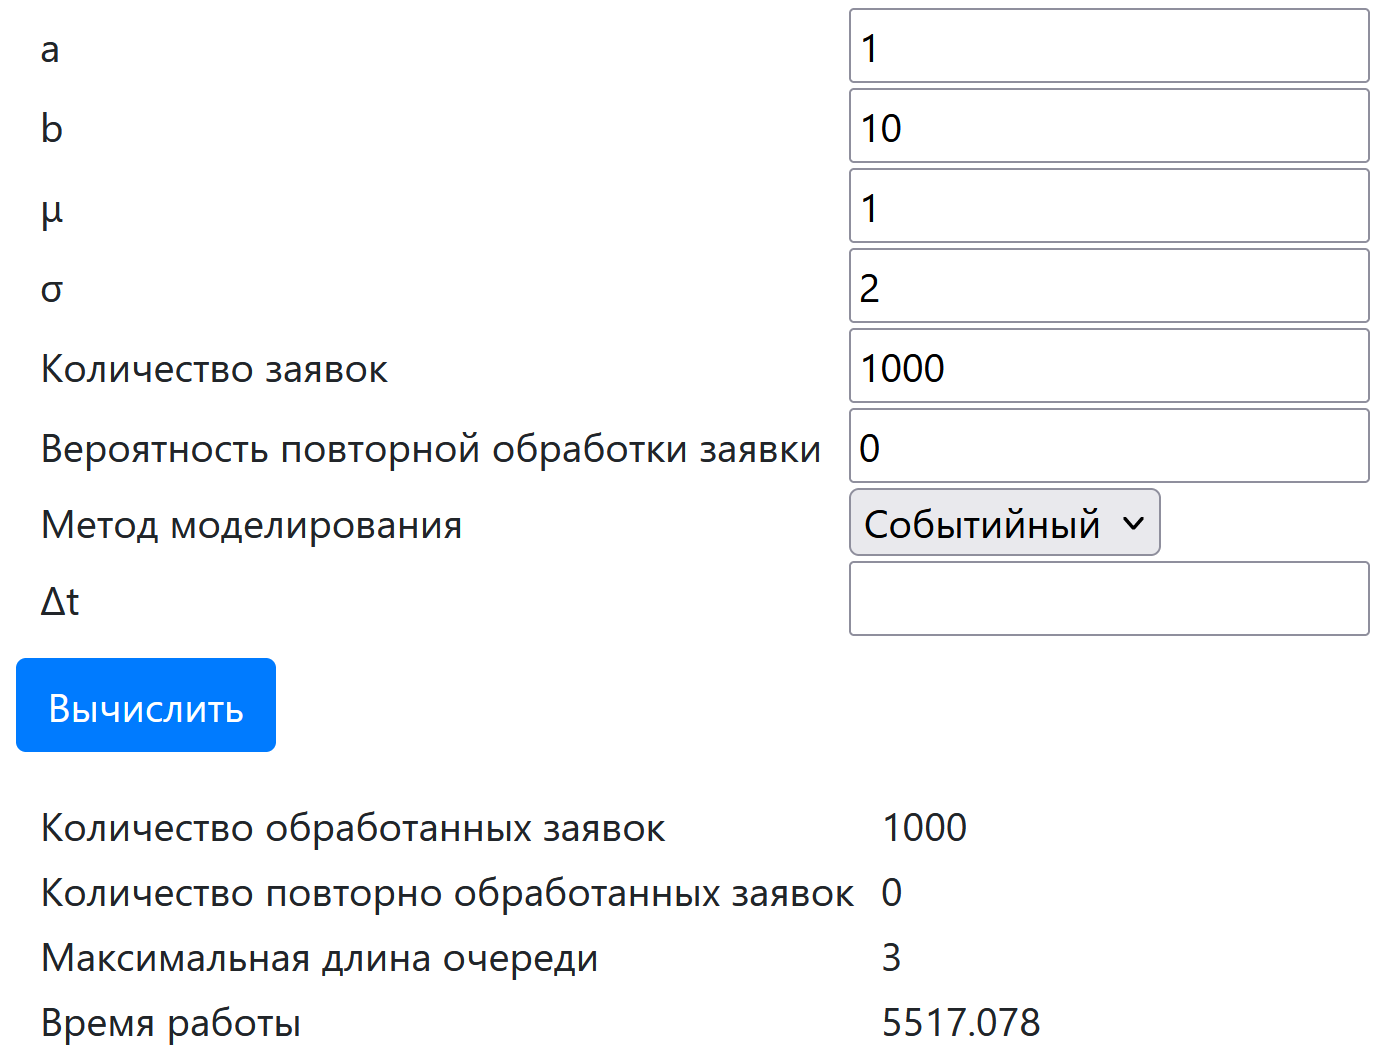
\includegraphics[scale=0.7]{1}
	\centering\caption{Событийный подход, вероятность возврата заявки в очередь равна 0}
\end{figure}
\begin{figure}[h!]
	\centering 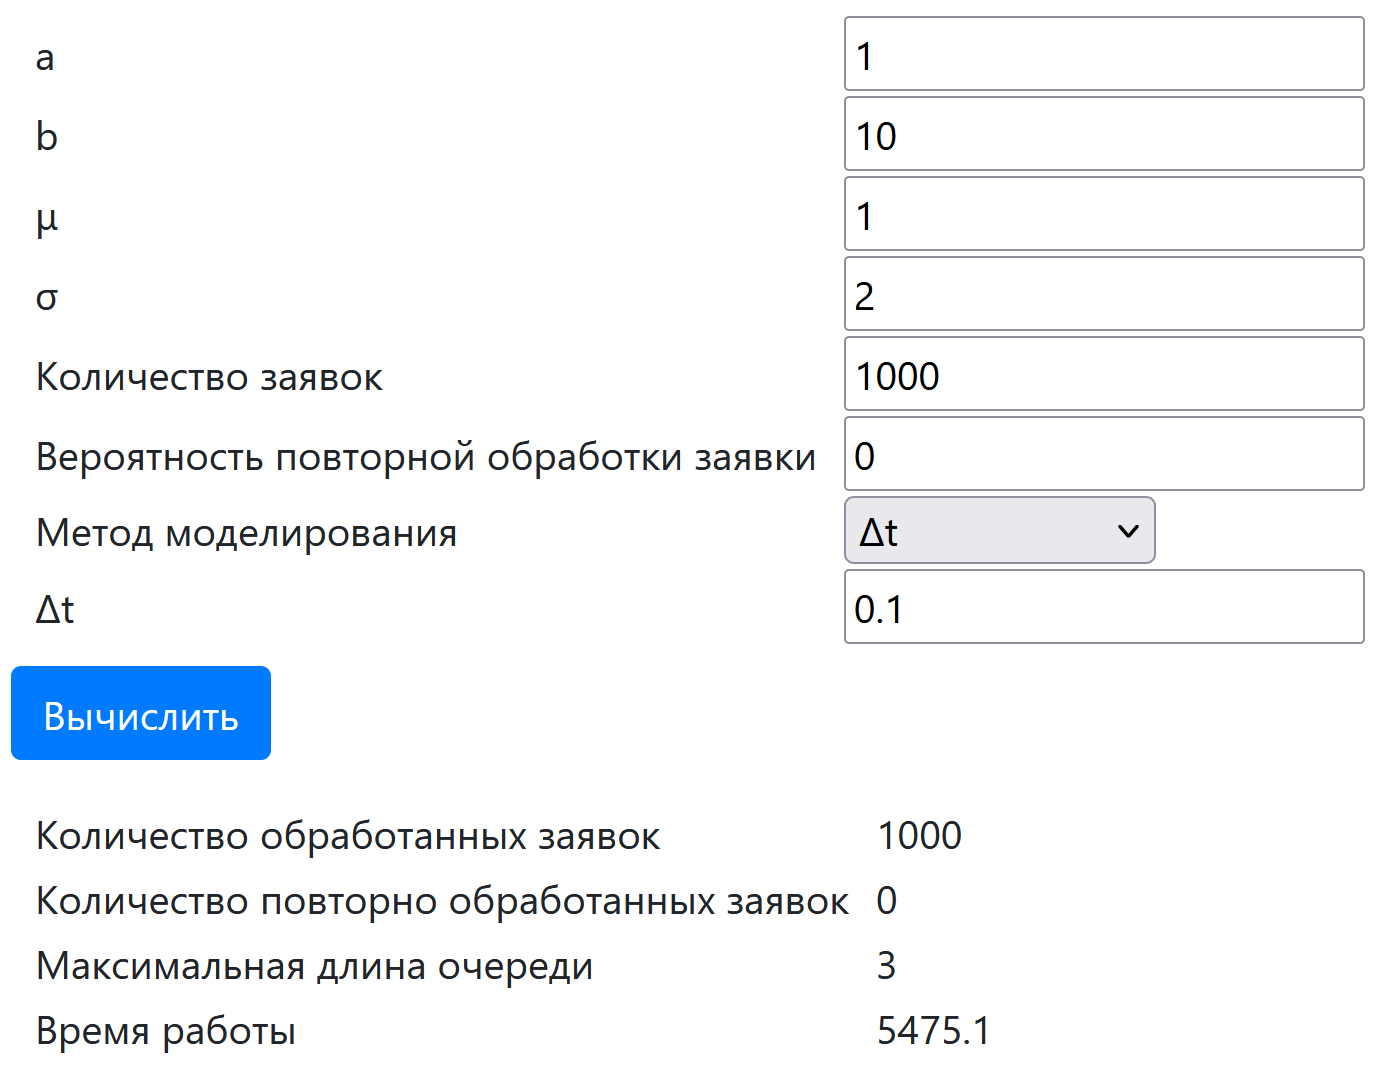
\includegraphics[scale=0.7]{2}
	\centering\caption{Пошаговый подход, вероятность возврата заявки в очередь равна 0}
\end{figure}
\clearpage
\newpage
\begin{figure}[h!]
	\centering 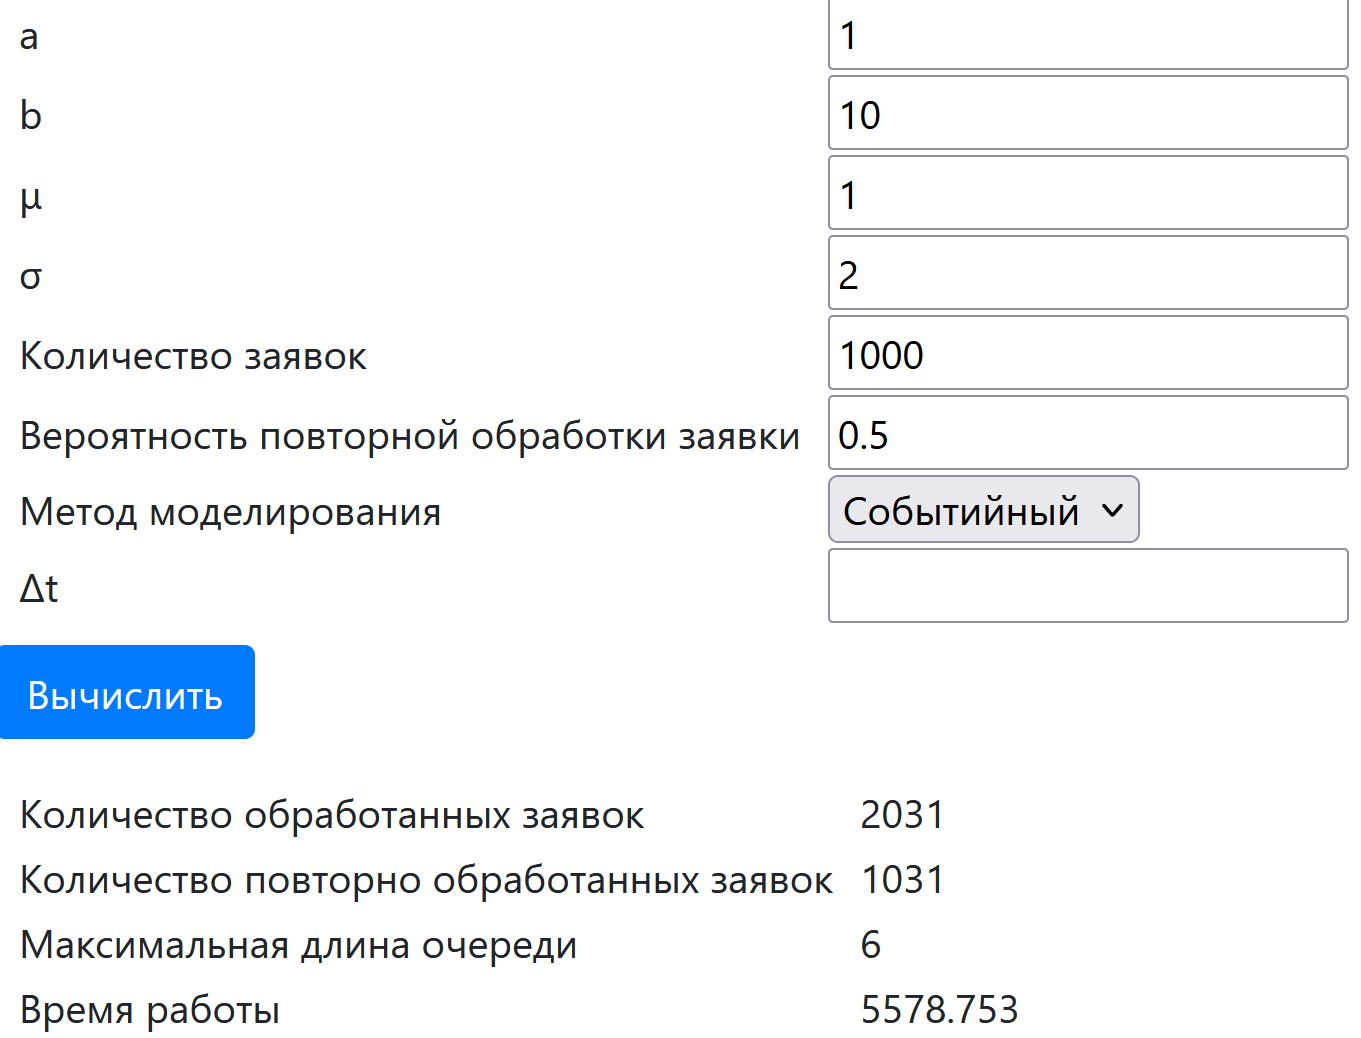
\includegraphics[scale=0.7]{3}
	\centering\caption{Событийный подход, вероятность возврата заявки в очередь равна 0.5}
\end{figure}
\begin{figure}[h!]
	\centering 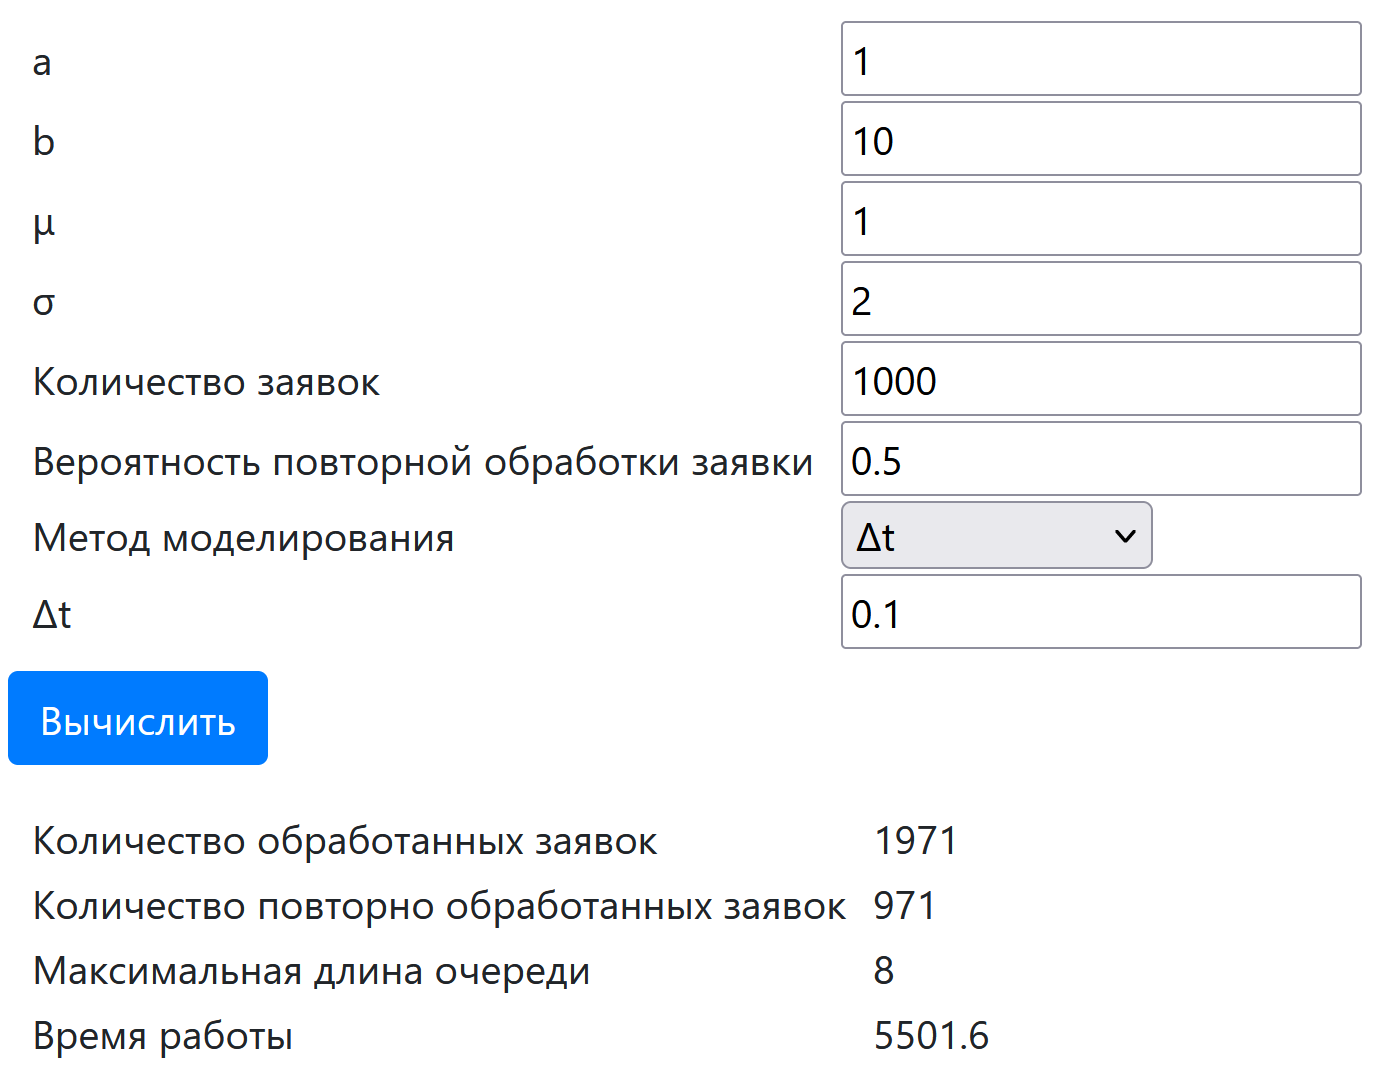
\includegraphics[scale=0.7]{4}
	\centering\caption{Пошаговый подход, вероятность возврата заявки в очередь равна 0.5}
\end{figure}
\clearpage
\newpage
\begin{figure}[h!]
	\centering 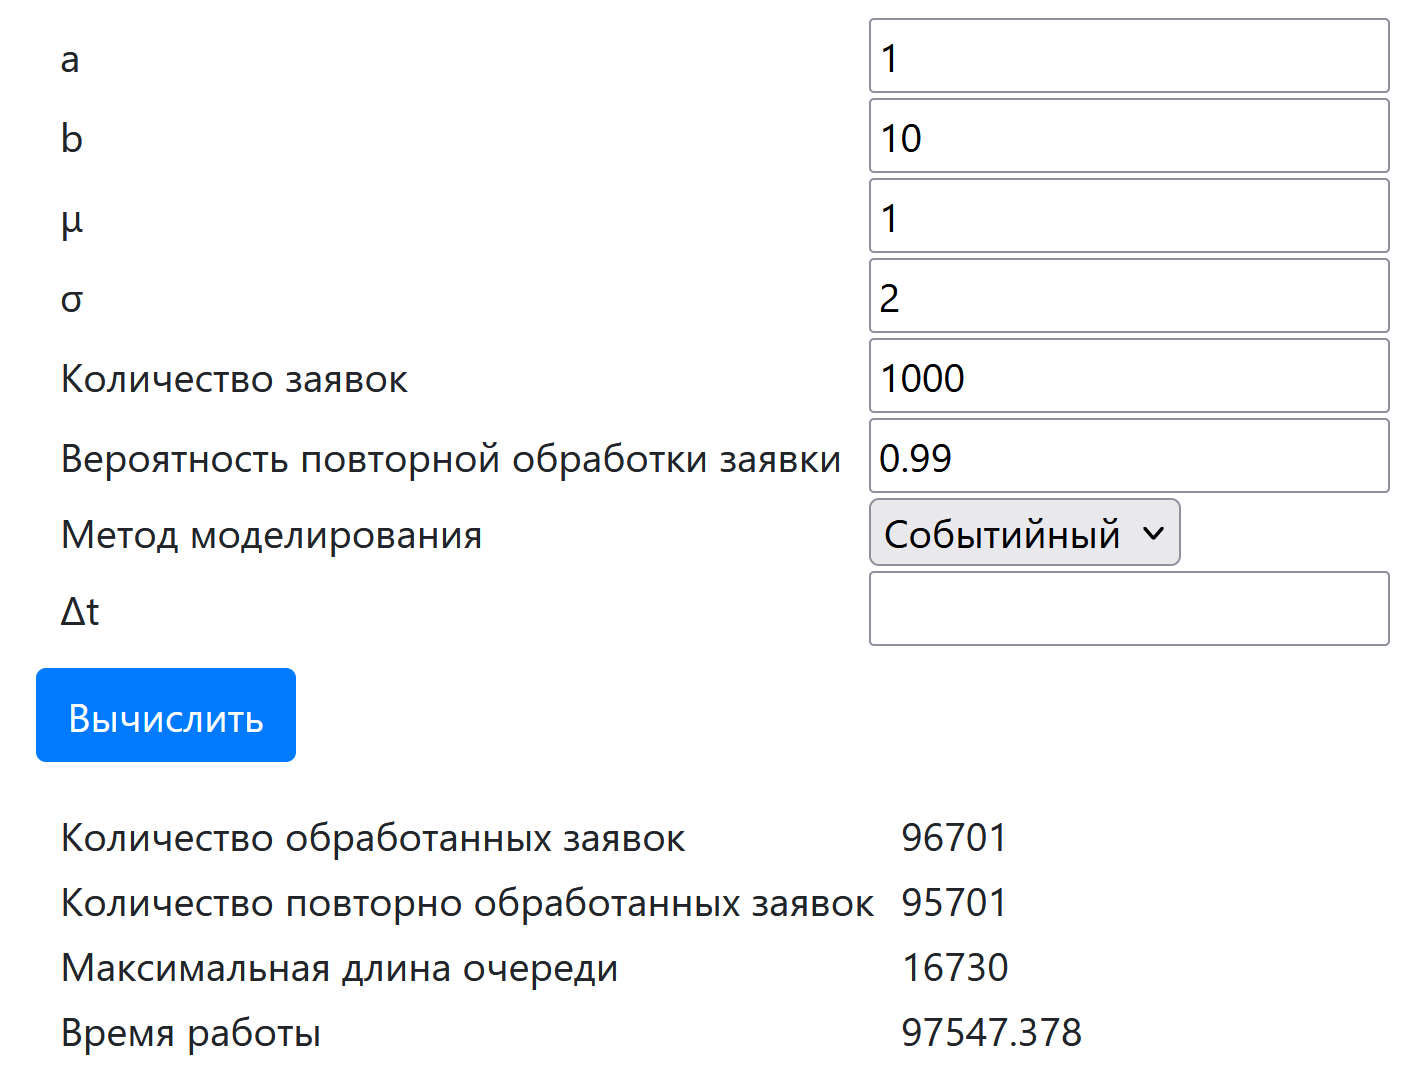
\includegraphics[scale=0.7]{5}
	\centering\caption{Событийный подход, вероятность возврата заявки в очередь равна 0.99}
\end{figure}
\begin{figure}[h!]
	\centering 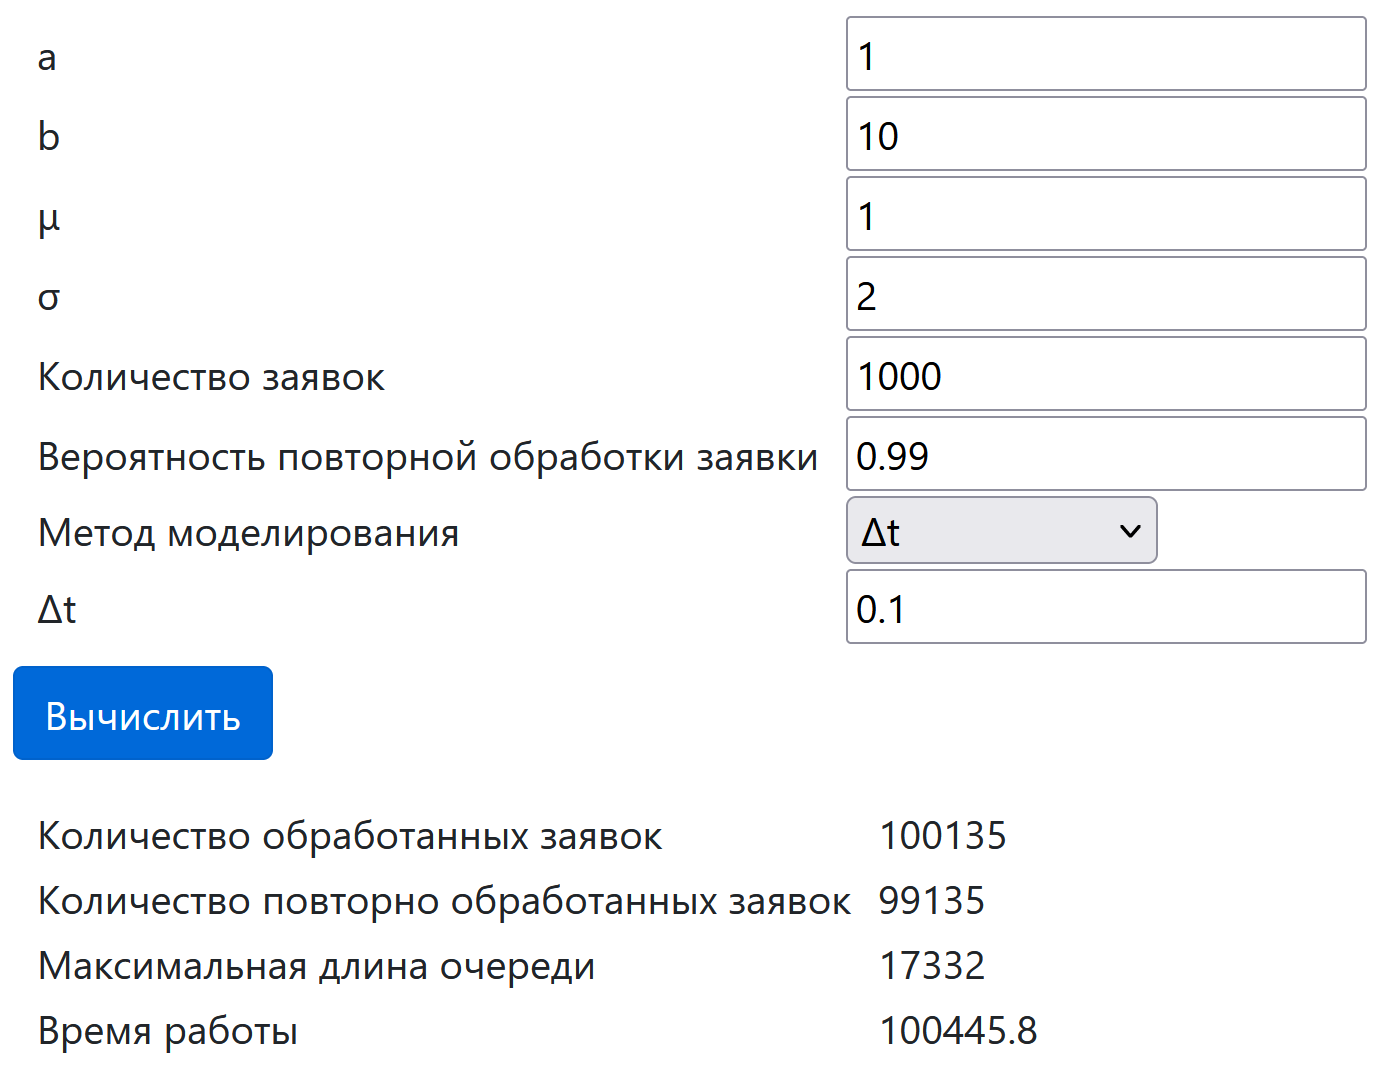
\includegraphics[scale=0.7]{6}
	\centering\caption{Пошаговый подход, вероятность возврата заявки в очередь равна 0.99}
\end{figure}
\clearpage
\newpage
\section{Листинг кода}
\definecolor{codegreen}{rgb}{0,0.6,0}
\definecolor{codegray}{rgb}{0.5,0.5,0.5}
\definecolor{codepurple}{rgb}{0.58,0,0.82}
\definecolor{backcolour}{rgb}{0.95,0.95,0.92}

\lstdefinestyle{mystyle}{
	backgroundcolor=\color{backcolour},   
	commentstyle=\color{codegreen},
	keywordstyle=\color{magenta},
	numberstyle=\tiny\color{codegray},
	stringstyle=\color{codepurple},
	basicstyle=\ttfamily\footnotesize,
	breakatwhitespace=false,         
	breaklines=false,                 
	captionpos=b,                    
	keepspaces=true,                 
	numbers=left,                    
	numbersep=5pt,                  
	showspaces=false,                
	showstringspaces=false,
	showtabs=false,                  
	tabsize=4
}

\lstset{style=mystyle}

\begin{lstlisting}[language=Python, caption = Программная реализация обслуживающего аппарата]
class Uniform:
	def __init__(self, a, b):
		if not 0 <= a <= b:
			raise ex.ParameterError("Parameters must be 0 <= a <= b")
		self._a = a
		self._b = b

	def generate(self):
		return nr.uniform(self._a, self._b)


class Normal:
	def __init__(self, mu, sigma):
		self._mu = mu
		self._sigma = sigma

	def generate(self):
		return nr.normal(self._mu, self._sigma)
		
class Generator:
	def __init__(self, generator):
		self._generator = generator
		self._receivers = set()
	
	def add_receiver(self, receiver):
		self._receivers.add(receiver)
	
	def remove_receiver(self, receiver):
		try:
			self._receivers.remove(receiver)
		except KeyError:
			pass
	
	def next_time(self):
		return self._generator.generate()
	
	def emit_request(self):
		for receiver in self._receivers:
			receiver.receive_request()
			
class Modeller:
	def __init__(self, uniform_a, uniform_b, n_mu, n_sigma, reenter_prop):
		self._generator = Generator(Uniform(uniform_a, uniform_b))
		self._processor = Processor(Normal(n_mu, n_sigma), reenter_prop)
		self._generator.add_receiver(self._processor)

	def event_based_modelling(self, request_count):
		generator = self._generator
		processor = self._processor

	gen_period = generator.next_time()
	proc_period = gen_period + processor.next_time()
	while processor.processed_requests < request_count:
		if gen_period <= proc_period:
			generator.emit_request()
			gen_period += generator.next_time()
		if gen_period >= proc_period:
			processor.process()
			if processor.current_queue_size > 0:
				proc_period += processor.next_time()
			else:
				proc_period = gen_period + processor.next_time()

	return (processor.processed_requests, processor.reentered_requests,
			processor.max_queue_size, round(proc_period, 3))

	def time_based_modelling(self, request_count, dt):
		generator = self._generator
		processor = self._processor

		gen_period = generator.next_time()
		proc_period = gen_period + processor.next_time()
		current_time = 0
		while processor.processed_requests < request_count:
			if gen_period <= current_time:
				generator.emit_request()
				gen_period += generator.next_time()
			if current_time >= proc_period:
				processor.process()
				if processor.current_queue_size > 0:
					proc_period += processor.next_time()
				else:
					proc_period = gen_period + processor.next_time()
			current_time += dt
	
		return (processor.processed_requests, processor.reentered_requests,
				processor.max_queue_size, round(current_time, 3))
\end{lstlisting}
\end{document}